\documentclass[11pt]{article}
\usepackage{graphicx}
\pagestyle{empty}
\usepackage[urlcolor=blue,colorlinks=true]{hyperref}

\title{GF Resource Grammar Summer School}
\author{Gothenburg, 17-28 August 2009}
\begin{document}

\begin{center}
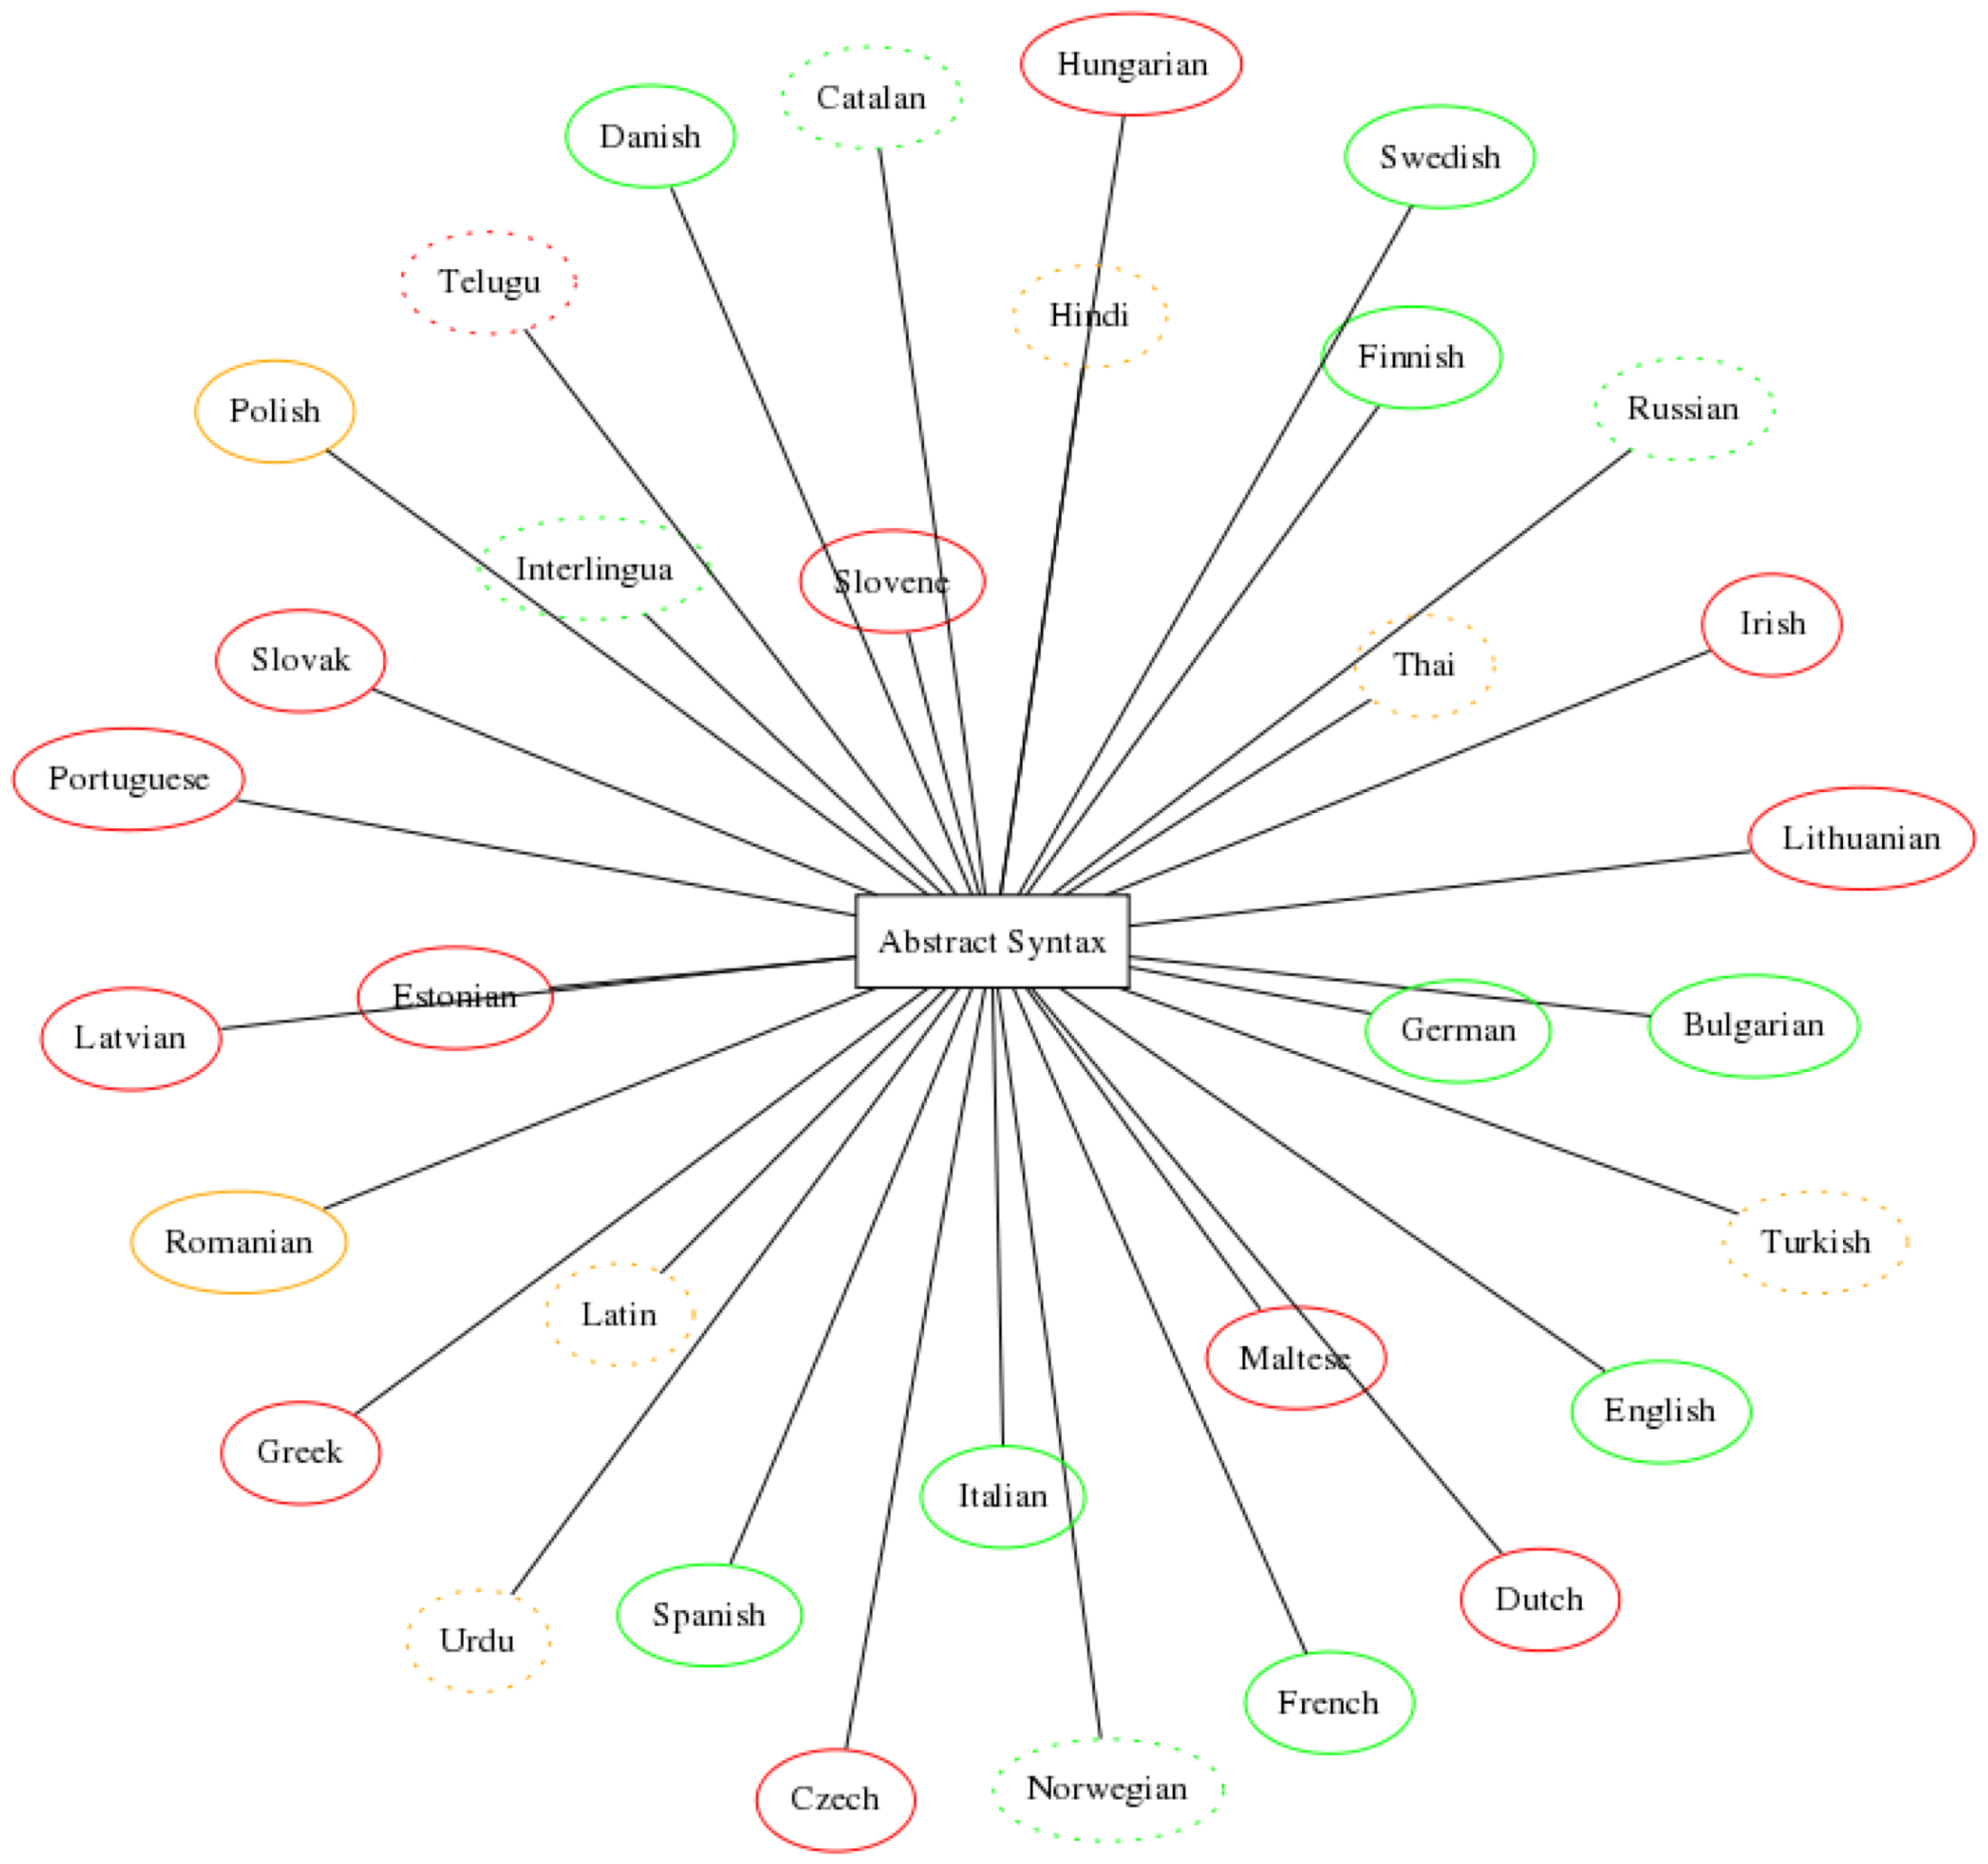
\includegraphics{summer-langs.png}

\vspace{3mm}

{\Large\bf GF Resource Grammar Summer School}

\vspace{2mm}

Gothenburg, 17-28 August 2009

\vspace{3mm}

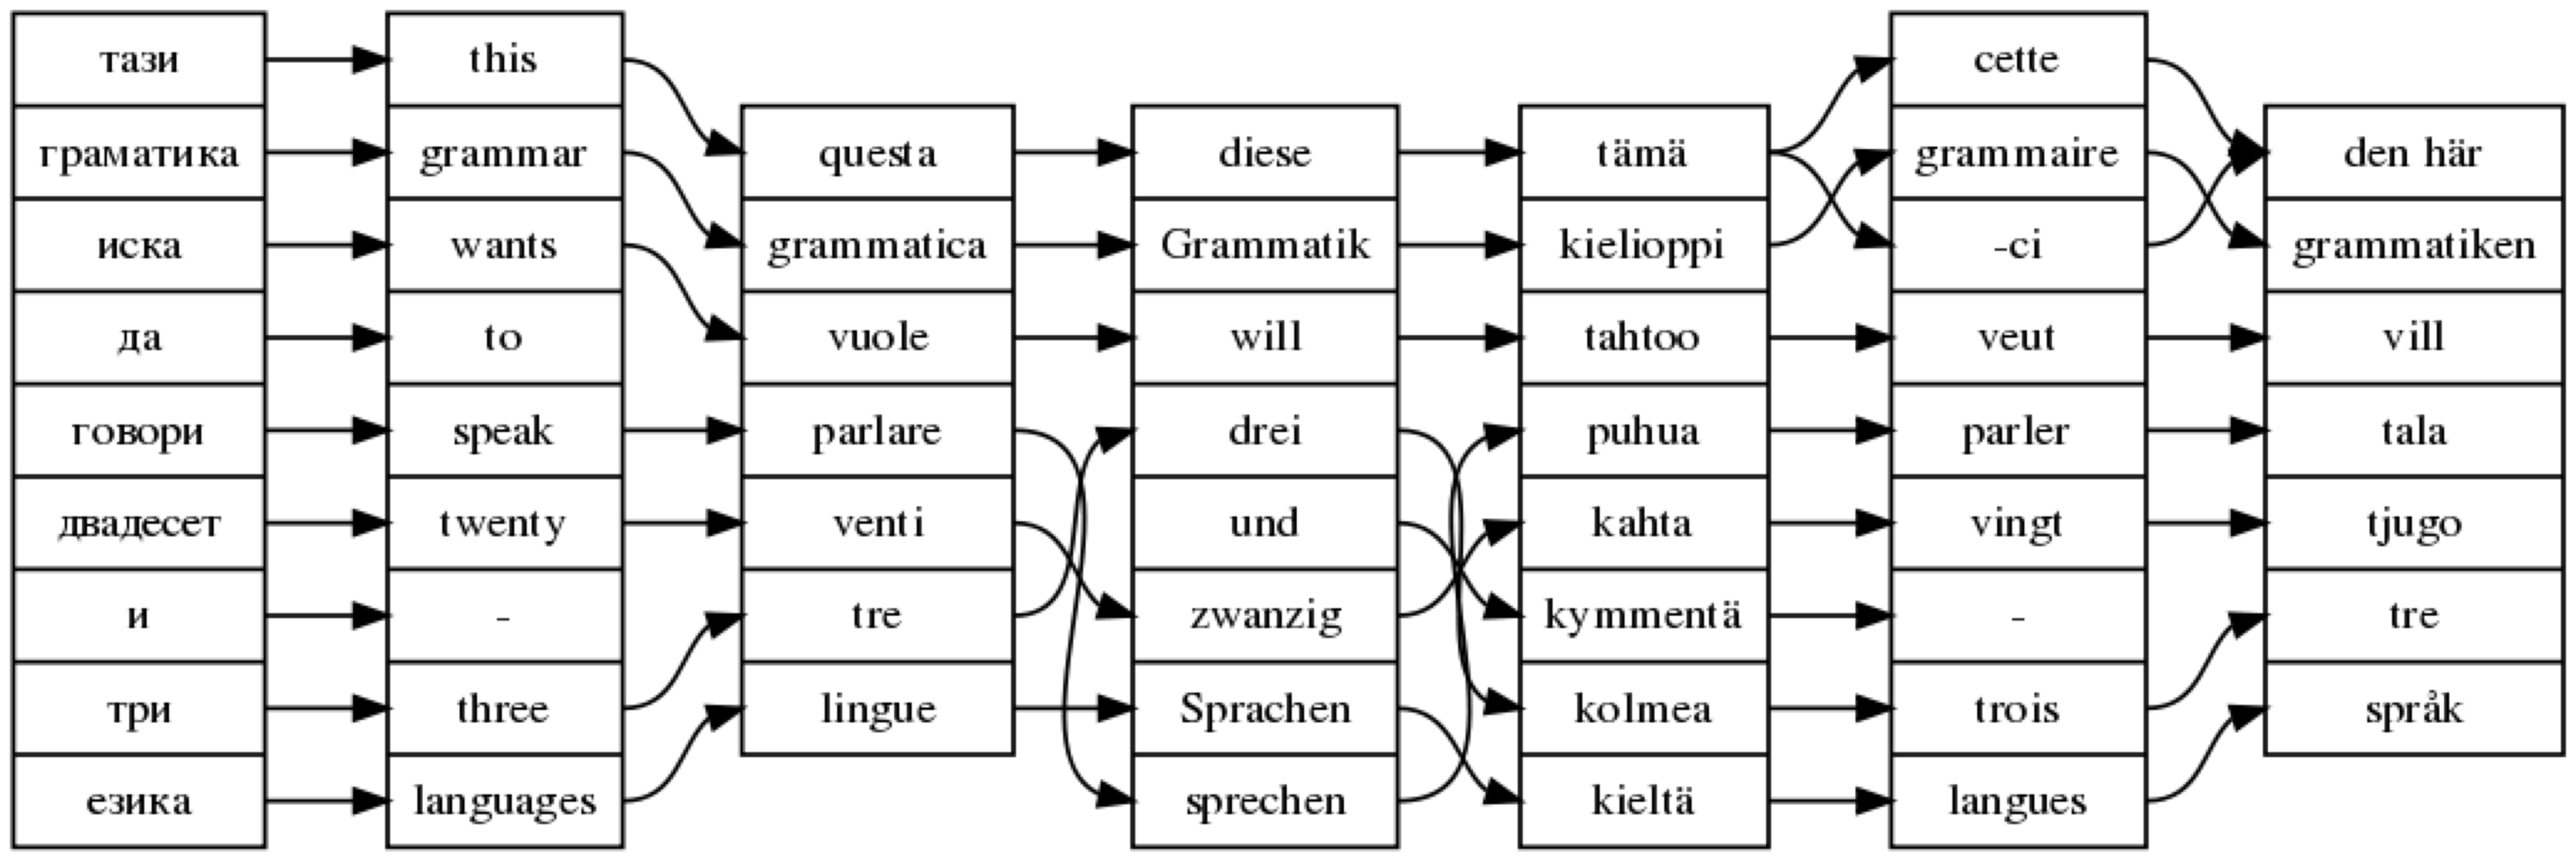
\includegraphics{summer-align.png}
\end{center}

\newpage

\begin{itemize}
\item Do you like programming? 
\item Are you interested in how your language really works? 
\item Would you like to try and build a computational grammar for your language, 
  and make it available as a part of an international open-source 
  programming effort? 
\end{itemize}

Then you should consider attending the GF Resource Grammar Summer School 
in Gothenburg on 17-28 August 2009.

The GF Resource Grammar Library is an open-source computational grammar resource
that currently covers 12 languages. The Summer School is a part of a 
collaborative effort to extend the library to all of the 23 official 
EU languages. Also other languages chosen by the participants are welcome.

The missing EU languages are: 
Czech, Dutch, Estonian, Greek, Hungarian, Irish, Latvian, Lithuanian,
Maltese, Portuguese, Slovak, and Slovenian. There is also more work to
be done on Polish and Romanian.

The linguistic coverage of the library includes the inflectional morphology
and basic syntax of each language. It can be used in GF applications
and also ported to other formats. It can also be used for building other
linguistic resources, such as morphological lexica and parsers.
The library is licensed under LGPL.

In the summer school, each language will be implemented by one or two students
working together. A morphology implementation will be credited
as a Chalmers course worth 7.5 ETCS points; adding a syntax implementation
will be worth more. The estimated total work load is 1-2 months for the
morphology, and 3-6 months for the whole grammar.

Participation in the summer school is free. 
Registration is done via the courses's Google group,

\begin{verbatim}
 http://groups.google.com/group/gf-resource-school-2009/
\end{verbatim}
The registration deadline is 15 June 2009.

Some travel grants will be available. They are distributed on the basis of a
GF programming contest in April and May.

For more information, see the Google Group above, as well as the 
Summer School web page,

\begin{verbatim}
 http://digitalgrammars.com/gf/doc/gf-summerschool.html
\end{verbatim}

% LaTeX2e code generated by txt2tags 2.4 (http://txt2tags.sf.net)
% cmdline: txt2tags summerschool-folder.txt
\end{document}
